\subparagraph{Configuration}\mbox{}\\

\begin{table}[H]
\centering
\begin{tabular}{|l|l|}
\hline
\textbf{Parameter} & \textbf{Value} \\
\hline
\multicolumn{2}{|c|}{\textbf{Training}} \\
\hline
Batch Size & 1 \\
\hline
Seed & 42 \\
\hline
Epochs & 15000 \\
\hline
Training Ratio & 0.9 \\
\hline
Number of Nodes & 1 \\
\hline
Gradient Clip Value & 1.0 \\
\hline
Metric to Monitor & val/recon\_loss \\
\hline
Metric Mode & Min \\
\hline
Device & CUDA \\
\hline
\multicolumn{2}{|c|}{\textbf{Model}} \\
\hline
Image Channels & 1 \\
\hline
Embedding Dimension & 8 \\
\hline
Number of Codes & 16384 \\
\hline
Number of Hidden Layers & 16 \\
\hline
Learning Rate & 5e-6 \\
\hline
Downsample Factors & [2, 2, 2] \\
\hline
Discriminator Channels & 64 \\
\hline
Discriminator Layers & 3 \\
\hline
Discriminator Iteration Start & 10000 \\
\hline
Discriminator Loss Type & Hinge \\
\hline
Image GAN Weight & 1.0 \\
\hline
Video GAN Weight & 1.0 \\
\hline
L1 Weight & 4.0 \\
\hline
GAN Feature Weight & 4.0 \\
\hline
Perceptual Weight & 4.0 \\
\hline
I3D Feature & False \\
\hline
Restart Threshold & 1.0 \\
\hline
No Random Restart & False \\
\hline
Normalization Type & Group \\
\hline
Padding Type & Replicate \\
\hline
Number of Groups & 32 \\
\hline
\multicolumn{2}{|c|}{\textbf{Dataset}} \\
\hline
Caching & Disk \\
\hline
Path & \url{/ravana/d3d\_work/micorl/data/ct\_images\_prostate\_32fixed/} \\
\hline
Image Size & 128 \\
\hline
Number of Slices & 32 \\
\hline
Window Width & 400 \\
\hline
Window Level & 60 \\
\hline
\end{tabular}
\caption{Configuration of the Medical Diffusion VQGAN.}
\label{table:meta_vqgan_params}
\end{table}

\subparagraph{Training}\mbox{}\\

The training was meant to last 15000 epochs, but it was manually stopped approximately at epoch 8000 due to the fact that for a long time model's reconstruction and perceptual loss did not change.

\begin{figure}[H]
\minipage{0.49\textwidth}
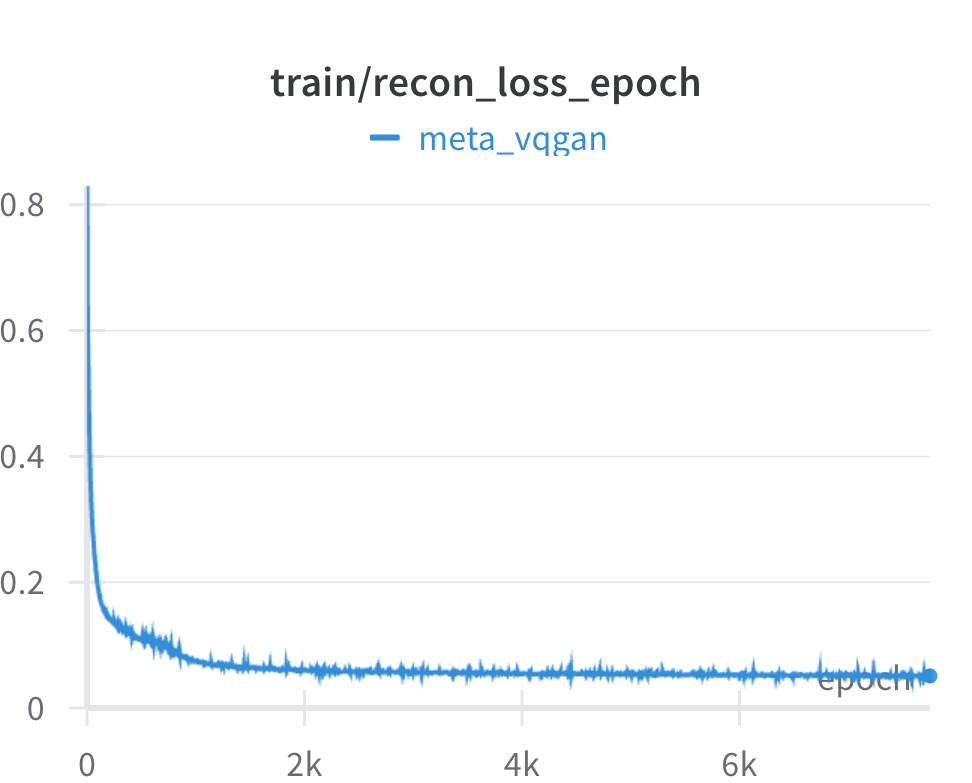
\includegraphics[width=\linewidth]{detailed_engineering/Meta VQGAN/charts/Section-2-Panel-13-1qhe42yar.png}
\caption{Reconstruction loss during the training.}
\endminipage\hfill
\minipage{0.49\textwidth}
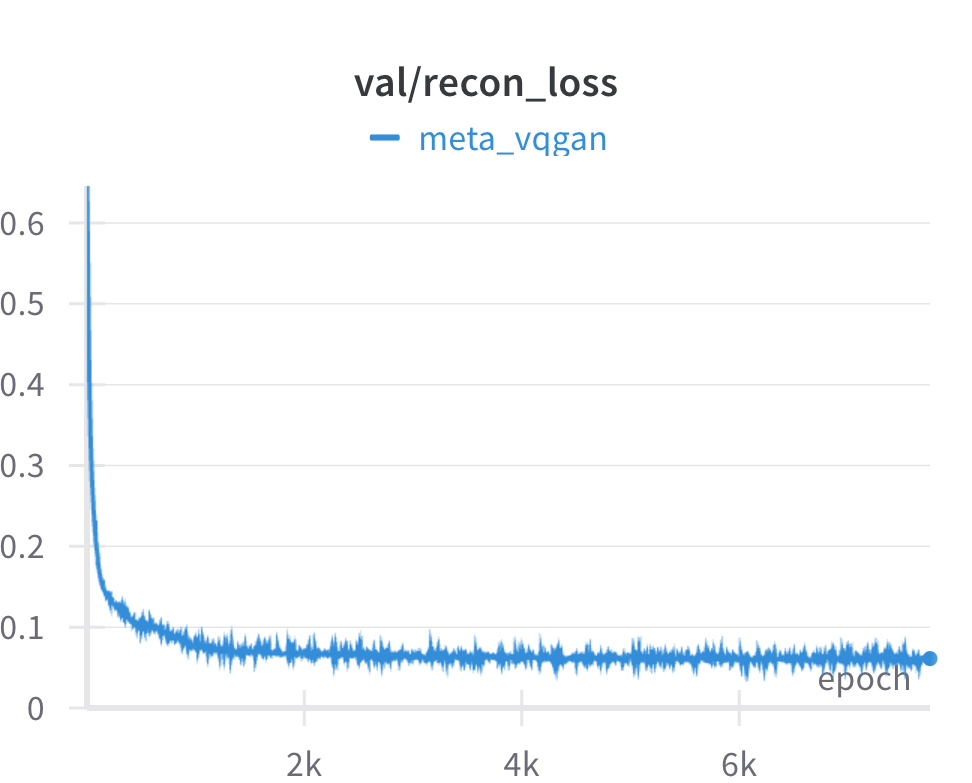
\includegraphics[width=\linewidth]{detailed_engineering/Meta VQGAN/charts/Section-4-Panel-3-hkj1c12xb.png}
\caption{Reconstruction loss during the validation.}
\endminipage
\caption{Reconstruction loss during the training and the validation. Lower is better.}
\end{figure}

\begin{figure}[H]
\minipage{0.49\textwidth}
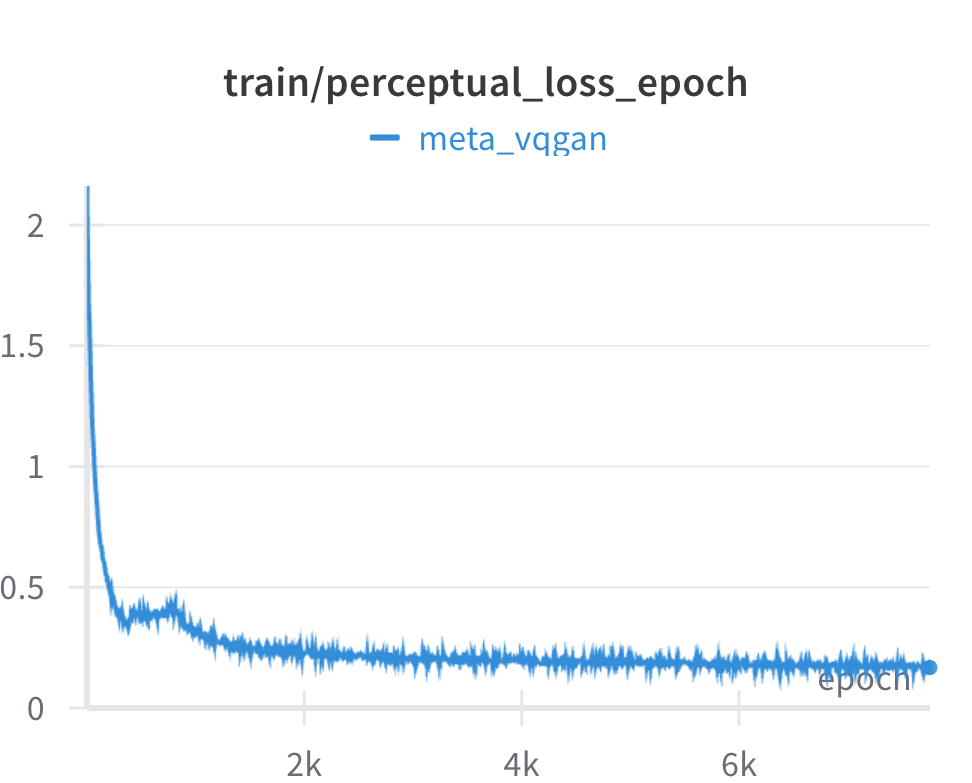
\includegraphics[width=\linewidth]{detailed_engineering/Meta VQGAN/charts/Section-2-Panel-7-jxu137h9u.png}
\caption{Perceptual loss during the training.}
\endminipage\hfill
\minipage{0.49\textwidth}
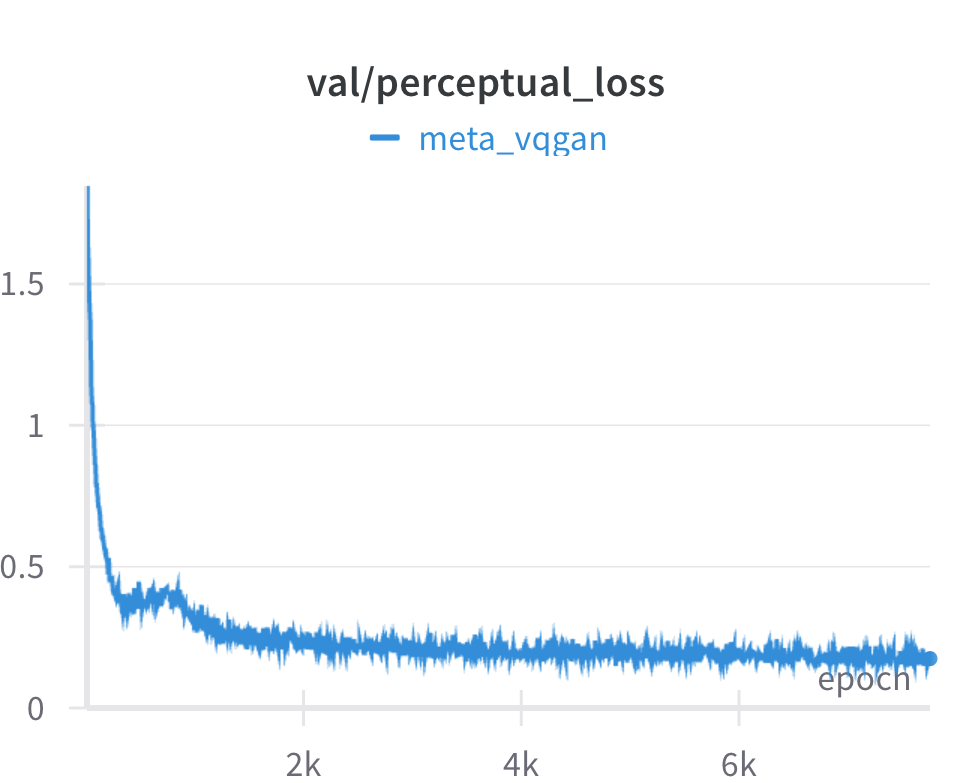
\includegraphics[width=\linewidth]{detailed_engineering/Meta VQGAN/charts/Section-4-Panel-0-9utd8c9z0.png}
\caption{Perceptual loss during the validation.}
\endminipage
\caption{Perceptual loss during the training and the validation. Lower is better.}
\end{figure}

\begin{figure}[H]
\minipage{0.49\textwidth}
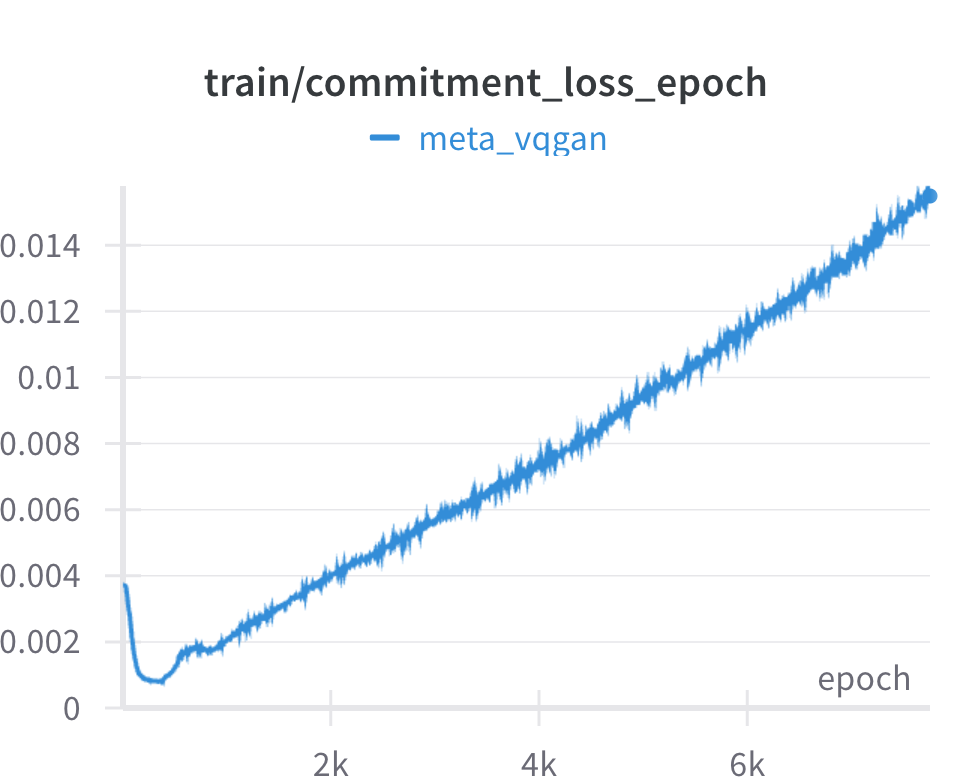
\includegraphics[width=\linewidth]{detailed_engineering/Meta VQGAN/charts/Section-2-Panel-11-4ox8mpc2c.png}
\caption{Commitment loss during the training.}
\endminipage\hfill
\minipage{0.49\textwidth}
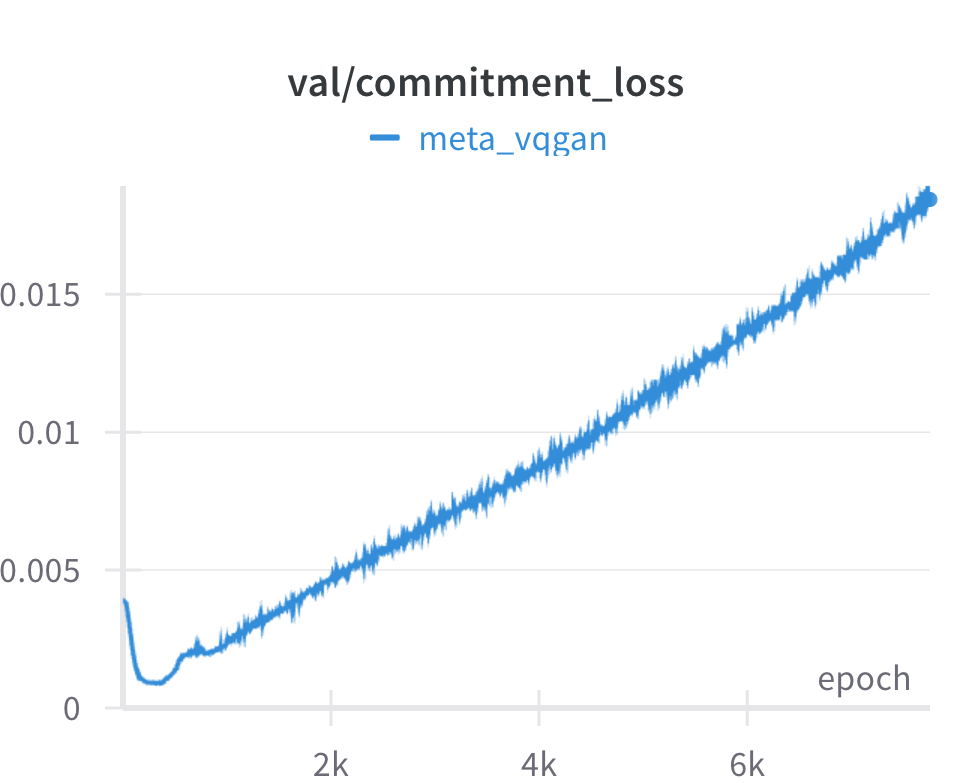
\includegraphics[width=\linewidth]{detailed_engineering/Meta VQGAN/charts/Section-4-Panel-2-2k8ixubhi.png}
\caption{Commitment loss during the validation.}
\endminipage
\caption{Commitment loss during the training and the validation.}
\end{figure}


\begin{figure}[H]
\minipage{0.49\textwidth}
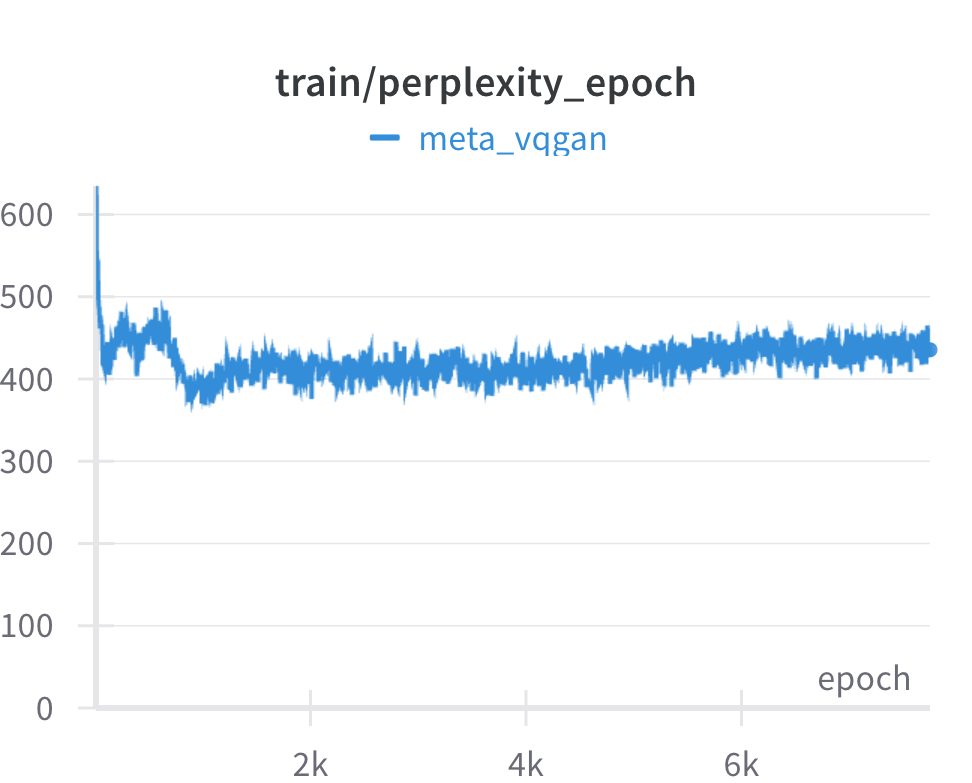
\includegraphics[width=\linewidth]{detailed_engineering/Meta VQGAN/charts/Section-2-Panel-1-5nrgzgmoj.png}
\caption{Perplexity during the training.}
\endminipage\hfill
\minipage{0.49\textwidth}
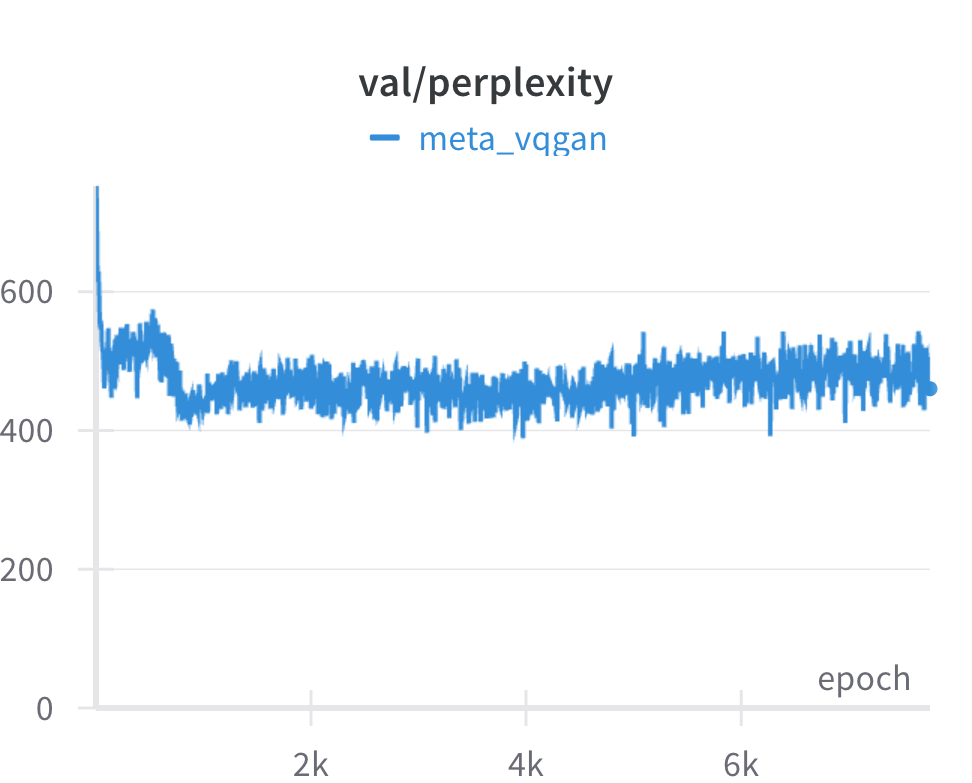
\includegraphics[width=\linewidth]{detailed_engineering/Meta VQGAN/charts/Section-4-Panel-1-njiwngfn7.png}
\caption{Perplexity during the validation.}
\endminipage
\caption{Codebook utilisation during the training and the validation. Lower is better.}
\end{figure}

\subparagraph{Results}\mbox{}\\

The training was finished with low reconstruction and perceptual losses. The resulting reconstruction $\hat{x}$ seems almost indistinguishable from the original $x$, as shown in the figure \ref{fig:md-vqgan-comparison}.

\begin{figure}[H]
    \centering
    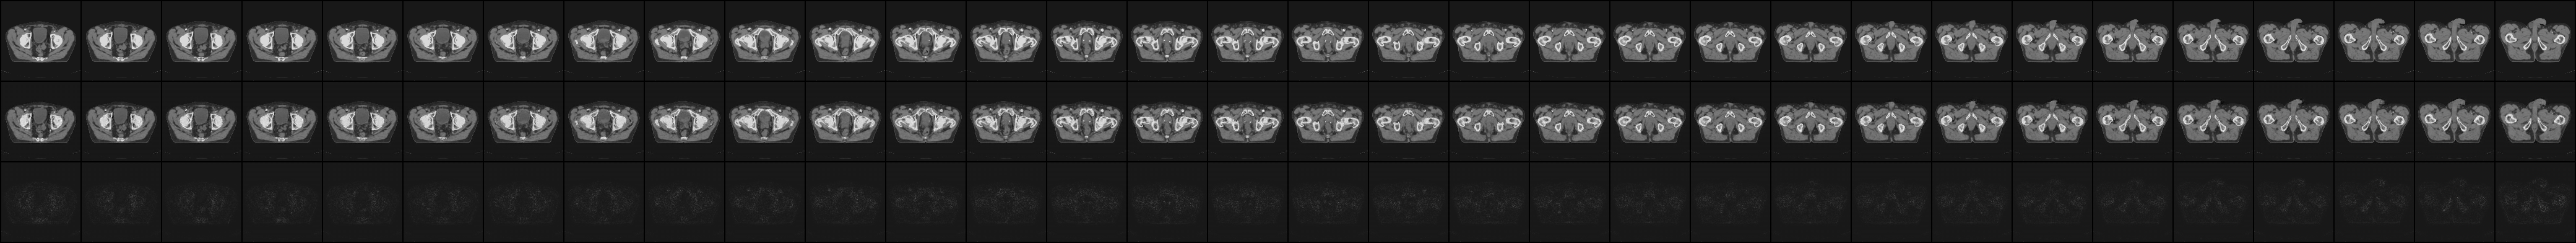
\includegraphics[width=\linewidth]{reports/meta_vqgan_reconstruction_comparison.png}
    \caption{Top - input, middle - reconstruction, bottom - difference.}
    \label{fig:md-vqgan-comparison}
\end{figure}

